\documentclass{article}
\usepackage{float}
\usepackage{textcomp}
\usepackage{graphicx}
\graphicspath{{images/}}
\usepackage{booktabs}
\usepackage{color}
\usepackage{verbatim}
\usepackage{listings}
\usepackage{underscore}
\setcounter{secnumdepth}{5}
\usepackage[bookmarks=true]{hyperref}
\author{Roberto Clapis (841859), Erica Stella (854443)} 
\date{\today}
\title{Politecnico di Milano
		\\A.A. 2015\@-\@2016
		\\Software Engineering 2: ``myTaxiService''
		\\\textbf{D}esign \textbf{D}ocument}
		\hypersetup{pdftitle={Design Document},    % title
		pdfauthor={Roberto Clapis, Erica Stella},                     % author
		pdfsubject={Design Document},                        % subject of the document
		pdfkeywords={TeX, LaTeX, taxi, DD, SoftwareEngineering2}, % list of keywords
		colorlinks=true,       % false: boxed links; true: colored links
		linkcolor=black,       % color of internal links
		citecolor=blue,       % color of links to bibliography
		filecolor=black,        % color of file links
		urlcolor=purple,        % color of external links
}
\begin{document}
\maketitle
\begin{center}
	
\includegraphics{polimi-logo}
\end{center}
\clearpage
\tableofcontents
\clearpage

\section{Introduction}
\subsection{Purpose}
\subsection{Scope}
\subsection{Definitions, Acronyms, Abbreviations}
\subsection{Reference Documents}
\subsection{Document Structure}

\section{Architectural Design}
\subsection{Overview}
\subsection{High Level Components and Their Interaction}
%TODO Descrizione alto livello di tutta l'architettura, e del sitema e di interazioni (molto HL)
\subsection{Component View}
%Mettere che la mobile app chiede cmq al webserver ma simula il fatto di avere tutto in cache tranne ciò che serve
\begin{figure}[H]
	  \makebox[\textwidth][c]{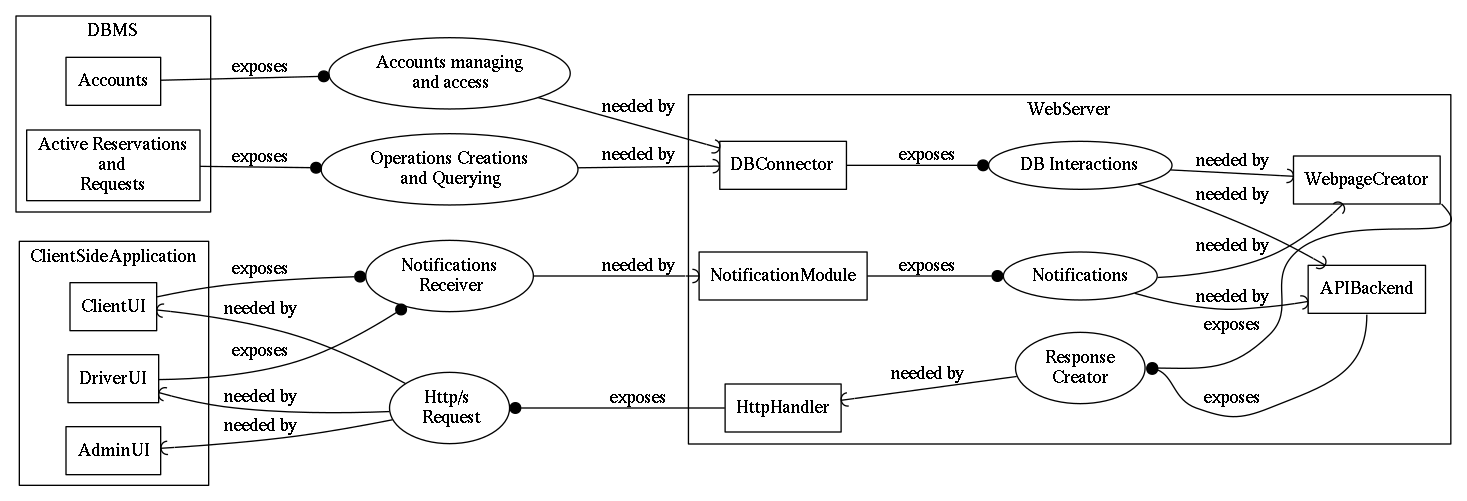
\includegraphics[width=1.4\textwidth]{Component}}%
\end{figure}
\clearpage
\subsection{Deployment View}
\begin{figure}[H]
	  \makebox[\textwidth][c]{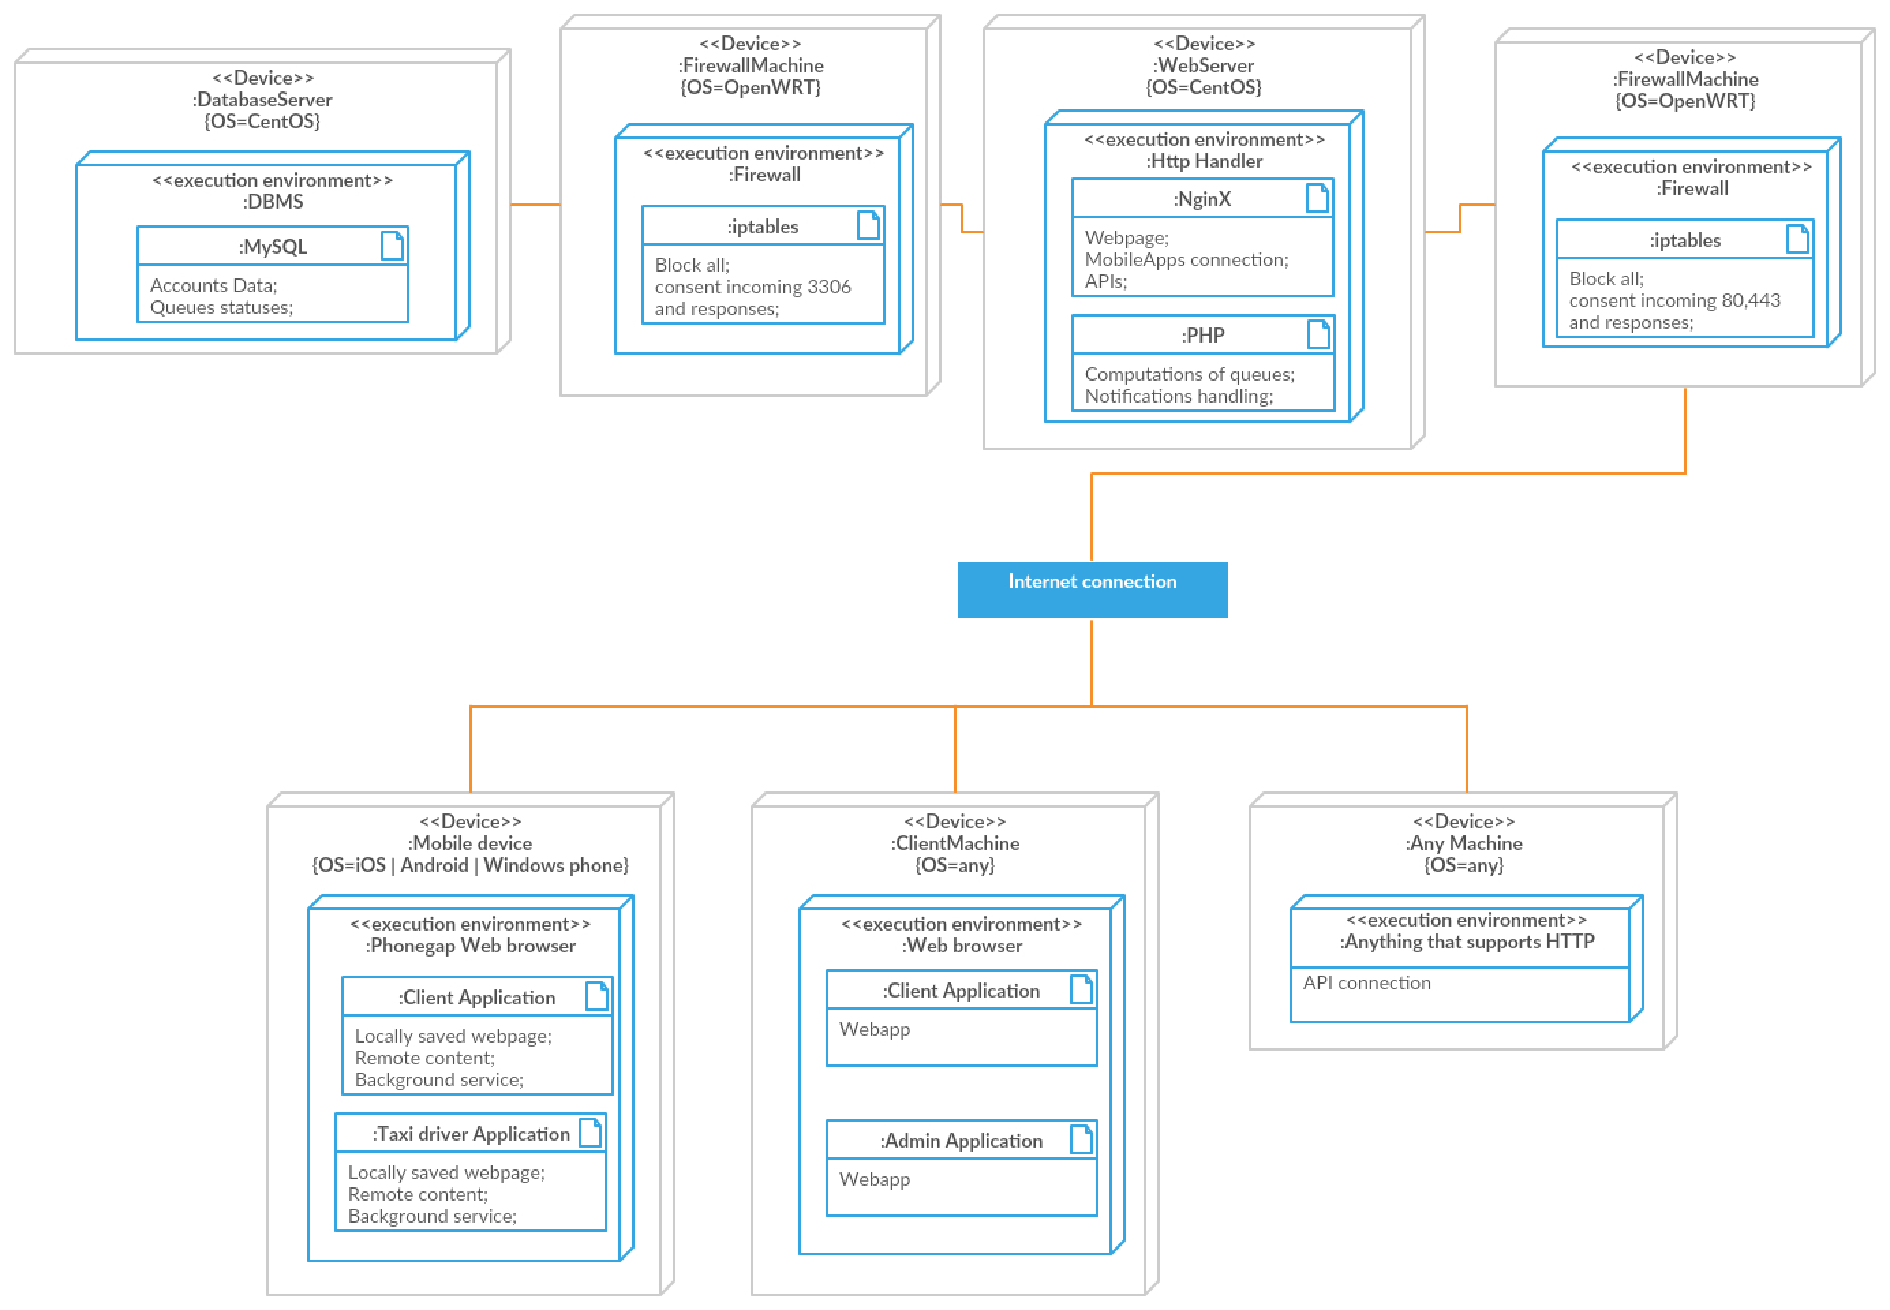
\includegraphics[width=1.3\textwidth]{Deployment}}%
\end{figure}
\begin{comment}
	A che livello di particolare lo faccio? 
	scendo fino al creare l'account e la chiamata o resto più ad alto livello? non saprei :/ sulla slide di riferimento non mi pare scenda molto ma vedi tu come pensi sia meglio
\end{comment}
\subsection{Runtime View}
%sequence diagram
%Request/alternative/%Cancel
%Registration
%Administrator modify
%Search for eta
\begin{comment}
	Di che casi farlo? quanto ricco? quanti devo farne?
\end{comment}
\subsection{Component Interfaces}
%dettagliare le cose della CV
\subsection{Selected Architectural Styles and Patterns}
%client-server
\subsection{Other Design Decisions}


\section{User Interface Design}
%nope

\section{Requirements Traceability}
%Explain	 how the requirements you have defined in  the RASD map	 into the design	 elements that you have  defined in this document

\section{References}
\clearpage
\section{Appendix}
Appendix for Roberto Clapis\\
Work hours: 15
\begin{center}
	Software Used:\\
	\-\\
	\begin{tabular}{*{2}{c}}
		\toprule
		Task & Software \\
		\midrule
		Edit \LaTeX\ Source & Vim\\
		Edit Graphs Sources & Vim\\
		Edit sources for Sequence Diagrams & Vim\\
		Convert Sequence Diagrams to images & Quick Sequence Diagram Editor\\
		Generate and Raster directed graphs& Dot\\
		Generate and Raster undirected graphs& Fdp\\
		General images mangling and cropping & ImageMagick \& Shotwell\\
		Convert \LaTeX\ source to PDF & \LaTeX\-MK\\
		Spell Check & Aspell \\
		\LaTeX\ Check & LaCheck\\
		\bottomrule
	\end{tabular}
\end{center}
\-\\
\-\\
\begin{comment}
TODO Erica
Appendix for Erica Stella\\
Work hours: 40
\begin{center}
	Software Used:\\
	\-\\
	\begin{tabular}{*{2}{c}}
		\toprule
		Task & Software \\
		\midrule
		Edit \LaTeX\ Source & TexStudio\\
		Use Case Diagrams & Eclipse\\
		Class Diagram & Eclipse\\
		General images mangling and cropping & GIMP\\
		Mockup & Pencil\\
		\bottomrule
	\end{tabular}
\end{center}
\end{comment}
\end{document}
